In order to understand from where comes the $\tilde{\Theta}(\sqrt{n})$ quantum
query complexity, it is mandatory to start by understanding the
Trichotomy theorem \cite{trichotomy_not_andris} and its dependency on Regular
languages and star free languages.
After that, to understand how to find a lower bounds, it is necessary to explore
the different adversary methods \cite{adversary_equivalence}.

\subsection{Quantum query for regular languages.}

In the article \cite{trichotomy_not_andris}, Aaronson, Grier and Schaeffer presented
a really interesting algebraic characterization of regular languages based on the
recognition by monoids and the syntactic congruence. This totally new to me definition
give me some hard time in order to understand it correctly.

\subsubsection{Regular languages}

Usually, the set of regular languages $\mathcal{R}$ on the alphabet $\Sigma$ is defined as the smallest
fixed point of the function F (the function that computes concatenations, unions, and Kleene stars)
including $\{\varnothing\} \cup \{\varepsilon\} \cup(\cup_{l\in\Sigma}\{l\})$
with F equal
\begin{align*}\label{eq:F}
    F(X) = & \{AB\  \forall (A,B)\in X^2\}                                                   \\
           & \cup \{A\cup B\ \forall (A,B) \in X^2 \}                                        \\
           & \cup \{A\cap B\ \forall (A,B) \in X^2 \}\ \texttt{\color{gray!50}$\#$ optional} \\
           & \cup \{A^*\ \forall A \in X \}.
\end{align*}

But here, the more convenient way to characterize regular language is with their
algebraic characterization. Indeed, a regular language is always a pre image of a subset
of a finite monoid under monoid homomorphism. A monoid is a 3-tuple of a set M, an
internal associative binary operation and finally the identity element associated to the
operation. A monoid homomorphism is a map from a monoid to another that preserve the
operation and the identity. Usually, to get the monoid representation of a regular
language, the first step is to compute the syntactic monoid. The syntactic monoid is
obtained by dividing $\Sigma^*$ by the following equivalence relation called syntactic
congruence
\[x \sim_L y \Leftrightarrow \forall (u, v) \in \left(\Sigma^*\right)^2, (uxv \in L \Leftrightarrow uyv \in L).\]
This equivalence relation is a congruence relation as the equivalence class can be multiplied
(i.e. if $x\sim_L y$ and $u \sim_L v$ then $xu \sim_L yv$). Now, it is necessary to get the monoid
homomorphism. For that it is sufficient to take the homomorphism that map an element to its
congruence class. Inside a congruence class, none or every element of the class is in $L$.
Indeed,  if $x$ is in $L$ and $x \sim_L y$ then for all
$(u, v)$ in $\left(\Sigma^*\right)^2, (uxv$ in $L \Leftrightarrow uyv$ in $L)$ thus
$x$ in $L$ implies $y$ in $L$ and finally as $x$ is in $L$ then $y$ is also in $L$.
Now, it is sufficient to prove that the syntactical monoid is of finite size\footnote{
    More precisely, the finiteness of the syntactic monoid is the property that
    characterize every regular languages. A good intuition to understand is first that it
    is always possible to construct finite automata from a finite monoid. For the second way,
    it is more delicate but the work done by Brzozozowski, Szykula and Ye \cite[2018]{Brzozowski}
    summarized a lot of result on the influence of the size of the minimal automata size on
    the size of the smaller syntactic monoid.}.

Finally, every regular language can be recognized by finite monoid.

\subsubsection{Star free languages}\label{ssec:starfree}

The set of star free languages is a really well studied subset of the regular languages.
Its definition differs a little from regular languages' one as the Kleene star is replace
by the complement operation (note $\overline{L}$). So star free languages are defined
as the smallest fixed point of the function F' (the function that computes concatenations, unions
and complements) and such that it includes
$\{\varnothing\} \cup \{\varepsilon\} \cup(\cup_{l\in\Sigma}\{l\})$.
This restriction does not imply that every star free language is finite. Indeed,
$\Sigma^*$ can be written $\overline{\varnothing}$. For example the language on
$\Sigma = \{1, 2, 3\}$ described with the regular expression $\Sigma^*20^*2\Sigma^*$ can be written
as following in the star free way
$\overline{\varnothing}2\overline{\overline{\varnothing}\Sigma{\setminus}\{0\}\overline{\varnothing}}2\overline{\varnothing}$.

As for regular languages, it exists an algebraic characterization for star free
languages. Let $M$ be a monoid, $M$ is said to be aperiodic if for every $x$ in
$m$ it exits a positive integer $n$ such that $x^n=x^n+1$. A theorem proved by
Schützenberger \cite{Schtzenberger1965OnFM} state that a language is recognized
by a finite aperiodic monoid if and only if if is star free.

Good examples of star free languages are the Dyck word languages with bounded heights.
It is first easy to have a finite automata that recognize Dyck word of height $k$ by
putting one state for each integer from 0 up to $k$. However, the belonging to the star
free regular languages is more delicate to prove. It has been done done by Italian
researcher in \cite[1978]{dyck_height_bound_star_free}.

\subsubsection{Trichotomy theorem}

\begin{theorem}[Aaronson, Grier and Schaeffer \cite{trichotomy_not_andris}]
    Every regular language has quantum query complexity
    \(0,\Theta(1), \tilde{\Theta}(\sqrt{n}),\) or \(\Theta(n) \)
    according to the smallest class in the following hierarchy that contains
    the language.
    \begin{itemize}
        \item Degenerate: One of the four languages \(\varnothing, \varepsilon, \Sigma^*\), or \(\Sigma^+\).
        \item Trivial: The set of languages which have trivial
              \footnote{A language $L$ is said to be trivial if and only if it exists 2 finite size alphabets
                  $L_1$ and $L_2$ such that $L = L_1 \Sigma^* L_2$.}
              regular expressions.
        \item Star free: The set of languages which have star-free regular expressions.
        \item Regular: The set of languages which have regular expressions.
    \end{itemize}
\end{theorem}

This theorem is really important as it give a good idea on the quantum query complexity
of many language recognitions. Moreover, the classes are now clearly defined so it is now
easier to know where is a problem compared to the classes in the introduction. However,
it does not give the exact quantum query complexity because for star free languages
the result is given using \(\tilde{\Theta}\). The $\tilde{\Theta}(\sqrt{n})$ means that
the quantum query complexity of any star free regular language is in
$\Theta(\sqrt{n}(\log_2(n))^p)$ for some $p$ a non negative constant.
As it is known that \Dyck{k} languages are star free, it is an interesting problem
to find the power of $\log_2(n)$ depending on the value of $k$.

\subsection{The bounds for \Dyck{k,n} problem}

The trichotomy theorem state that \Dyck{k,n} language has a quantum query complexity
in $\tilde{\Theta}(\sqrt{n})$. The $\Theta$ means that the best possible algorithm
is both a $\tilde{O}(\sqrt{n})$ and a $\tilde{\Omega}(\sqrt{n})$. So, a common method
to find the power of $\log_2(n)$ depending on $k$ is the squeeze theorem. More
precisely, the quantum query complexity of \Dyck{k, n} is trapped between a lower
and an upper bound for quantum query complexity. So it is possible to deduce
the quantum query complexity from an increasing sequence of lower bound and
a decreasing sequence of upper bound such that they share the same limit $l$ with $l$
equals to $Q(\Dyck{k,n})$. How to find this sequence ?
\begin{itemize}
    \item \textbf{For the lower bound sequence.} Some of the most important tools to compute
          lower bounds are called \textbf{quantum adversary methods} and have been invented by Ambainis
          \cite{andris_adversary_methode}. This tools can compute
          lower bounds more or less tight and some of this adversary methods have really
          useful property such as being compatible with a certain type of composition
          of problems. This lead to the \textbf{reduction methods} that can compute
          a lower bounds from different but easier problem's ones.
    \item \textbf{For the upper bound sequence.} The main method is to \textbf{find quantum
              query algorithms} that are more and more efficient. An other way is also
          \textbf{by reduction} to a more difficult problem with a
          good enough upper bound.
    \item \textbf{For the same limit.}
          The idea is to do an iterative process where each step improves successively
          each bound until only one will continue to be improved. Finally, both
          bounds may end up matching. However, before my internship, both \Dyck{k,n}'s
          lower and upper bounds where stuck to $\Omega\left(c^k\sqrt{n}\right)$ for some
          constant $c$ greater than 1 and $O\left(\sqrt{n}\left(\log_2(n)\right)^{0.5k}\right)$.
\end{itemize}


\subsubsection{Lower bound on the quantum query complexity of \Dyck{k, n}}

\paragraph*{\textbf{The quantum adversary methods:}}
This part as for goal to present some quantum adversary methods and their usages.

\subparagraph*{\textbf{The adversary method.}} The adversary method is a classical
way to prove lower bound in classical algorithmic. Indeed, the idea behind the classical
adversary is to prove that for every algorithm, it exist an entry such that the algorithm
cannot decide in less unit of complexity than the lower bounds. In general, during
the algorithm execution, the adversary modifies entry values that have not been already used
in order to increase the execution time. This classical adversary work great for classical
algorithm but is not really useable on  quantum algorithms.

\subparagraph*{\textbf{The super basic quantum adversary method.}}
In order to recognize a language it is mandatory to be able to distinguish between
a valid word $v$ and an invalid word $w$. So at the output of the quantum query
algorithm, the states $\ket{\psi^T_v}$ and $\ket{\psi^T_w}$ should be distinguishable thus
$\vert \langle \psi_v^T \vert \psi_w^T \rangle \vert < \frac{2}{3}$. How do they
will differs? The quantum query algorithm start with
$\ket{\psi^0_v} = \ket{\psi^0_w} = \ket{\psi_{start}}$. Moreover, the inner product
of both states isn't affected by $U_i$ gates because there are unitary. However, the $Q_i$
gates affect this inner product as the $Q_i$'s behaviors are depending on the input.
Let define the progress measure $\mathcal{P}$ such that
$\mathcal{P}(t) := \langle \psi_v^t \vert \psi_w^t \rangle$ where $\ket{\psi^t}$ represents
the state after $Q_t$. Let suppose it exists $d$ such that for all $0\leq t \leq T-1$,
$\vert \mathcal{P}(t+1)-\mathcal{P}(t)\vert \leq d$. It implies the following inequality
\[
    \mathcal{P}(T) = \underbrace{\mathcal{P}(0)}_{=1} + \sum_{i=0}^{T-1}\underbrace{\mathcal{P}(i+1)-\mathcal{P}(i)}_{\geq -d}  \geq \mathcal{P}(0) - T\times d.
\]
Moreover, $\mathcal{P}(T)$ should be lower than $\frac{2}{3}$ so it implies that
$1 - T\times d$ should also be lower than $\frac{2}{3}$ and finally that
$T$ should be a $O(\frac{1}{d})$. This give a general idea of how to determined
a lower bound but it isn't precise enough to get a theorem. In its courses,
Ryan O'Donnell \cite{Odonnel_course} explained a simple to understand adversary method called the super
basic adversary method. This adversary allow to compute a lower bound
by using the following method:

\begin{theorem}
    Let define $YES$ the set equal to $f^{-1}(accepted)$ and $NO$ the set
    equal to

    $f^{-1}(rejected)$. If it exist two subset $Y\subseteq YES$ and
    $Z \subseteq NO$ such that:
    \begin{itemize}
        \item For each $y$ in $Y$, there are at least $m$ strings $z$ in $Z$ with dist$(y,z)=1$.
        \item For each $z$ in $Z$, there are at least $m'$ strings $y$ in $Y$ with dist$(y,z)=1$.
    \end{itemize}
    Then the quantum query complexity $Q(f)$ is in  $\Omega(\sqrt{m m'})$.
\end{theorem}


The proof of the theorem can be found in \autoref{proof:advmethod}.
One important result of the adversary method is the lower bound on the quantum query complexity
of $Ex_{2m}^{m \vert m+1}$
in $\Omega\left(m\right)$ where the problem $Ex_{2m}^{m\vert m+1}$ consists to
recognize between $|x|=2m\ \land\ |x|_1 = m$ , and $|x|=2m\ \land\ |x|_1 = m+1$.
More generally, the method of an adversary define a process to find the lower $d$ possible. The
super-basic adversary method as its name let suggest is simple but does not give
a tight lower bounds. For this, the method should be more complicated which results
in longer days on the board to find the parameters of the methods.

Let $f:D\to\{0,1\}$ be the function whose quantum query complexity is unknown. Two other adversary methods
are described as following:
\begin{itemize}
    \item \textbf{The Basic adversary method by Ambainis \cite{andris_adversary_methode}}.
          \begin{theorem}
              \label{th:basicadv}
              Let define $YES$ the set equal to $f^{-1}(accepted)$ and $NO$ the set
              equal to

              $f^{-1}(rejected)$. Moreover, let $Y\subseteq YES$, $Z \subseteq NO$, and
              let $\mathcal{R} \subseteq Y\times Z$ be a set of "hard to distinguish" pairs, such that:
              \begin{itemize}
                  \item For each $y$ in $Y$, there are at least $m$ strings $z$ in $Z$ with $(y,z)$ in $\mathcal{R}$.
                  \item For each $z$ in $Z$, there are at least $m'$ strings $y$ in $Y$ with $(y,z)$ in $\mathcal{R}$.
              \end{itemize}
              Also, let define $\mathcal{R}_i$ as a restriction from $\mathcal{R}$ such
              that $(y, z)$ is in $\mathcal{R}_i$ if and only if $(y, z)$ is in $\mathcal{R}$
              and $y_i \neq z_i$.
              In addition,
              \begin{itemize}
                  \item For each $y$ in $Y$ and $i$, there are at most $l$ strings $z$ in $Z$ with $(y,z)$ in $\mathcal{R}_i$
                  \item For each $z$ in $Z$ and $i$, there are at most $l'$ strings $y$ in $Y$ with $(y,z)$ in $\mathcal{R}_i$
              \end{itemize}
              Then the quantum query complexity $Q(f)$ is in  $\Omega(\sqrt{\frac{m m'}{ll'}})$.
          \end{theorem}
    \item \textbf{The general adversary method by Reichardt \cite{Reichardt_2009}}.

          A symmetric matrix $\Gamma$ is an adversary matrix for $f$ if the
          rows and cols of $\Gamma$ can be indexed by input $x$ in $D$ such that
          $\Gamma_{x,y} = 0$ if $f(x) = f(y)$. $\Gamma^{(i)}$ is defined from $\Gamma$
          and is a similarly sized matrix such that $\Gamma^{(i)}_{x,y} = \left\{
              \begin{array}{ll}
                  \Gamma_{x,y} & \textrm{if} \ x_i\neq y_i \\
                  0            & \textrm{otherwise}
              \end{array}
              \right.$. This two objects allow to define the following notion of adversary plus minus
          \[Adv^{\pm}(f) = \underset{\textrm{\shortstack{$\Gamma$ -
                          an adversary\\[-1ex] matrix for $f$}}}{\max} \frac{\Vert \Gamma\Vert }{\max_i \Vert \Gamma^{(i)}\Vert}.
          \]

          \begin{theorem}
              The adversary plus minus is such that $Q(f) = O(Adv^{\pm}(f))$.
          \end{theorem}

          In \cite{Reichardt_2009}, Reichardt gave the proof that the general adversary method
          is not only giving a lower bound to the quantum query complexity as the method
          return the directly the quantum query complexity of $f$.
\end{itemize}

All this adversary methods are really interesting to compute lower bounds, but sometime it is
useful to reuse already computed ones.


\paragraph*{\textbf{The reduction method:}}

For some problems, it looks obvious that some are easier than the others.
Computer scientists have developed tools to handle more formally this notion
of difficulty comparison. One of the main tool is named reduction. A reduction
is the process to solve a first problem using an algorithm for a second one.
Because the second problem is able to solve the first one, it is said to be
harder, which is written $P_1 \leq P_2$.
\begin{theorem}{Reduction and $Adv^{\pm}$}
    \[P_1 \leq P_2 \implies Adv^{\pm}(P_1) \leq Adv^{\pm}(P_2)\]
\end{theorem}
Finally, problems can also be composed. Lets take $P_1:\{0, 1\}^n \to \{0, 1\}$
and $P_2:\{0, 1\}^m \to \{0, 1\}$. Then $P_1 \circ P_2$ is defined as
\[(P_1 \circ P_2)(x_1 \ldots x_{nm}) := P_1\left(\underbrace{P_2(x_1\ldots x_m), \ldots, P_2(x_{(n-1)m+1}\ldots x_{nm})}_{n}\right).\]
This composition has a great behavior with the adversary plus minus.
\begin{theorem}{Composition and $Adv^{\pm}$}
    \[Adv^{\pm}(P_1 \circ P_2) \geq Adv^{\pm}(P_1)\times Adv^{\pm}(P_1)\]
\end{theorem}
Andris' team found that the $Ex_{2m}^{m\vert m+1}$ problem can be reduce using the OR and AND
problems to \Dyck{k} problem with the reduction described in \cite{art:2DGrid}. They finally
get a lower bound in $\Omega(c^k\sqrt{n})$ for the quantum query complexity of \Dyck{k,n}.

The team also gets another result (not published),
they have founded an upper bound using a reduction from
\Dyck{k,n} to a problem about the connectivity into a 2d
directed grid with missing edges. This upper bound of
$O(\sqrt{n}(\log_2(n))^{0.5(k-1)})$ is interesting as it
is an upper bound in $\tilde{\Theta}(\sqrt{n})$.

\subsubsection{Best known algorithm to recognize \Dyck{k, n}}
\label{already_known}

Before checking the algorithm for \Dyck{k,n}, it is necessary to define some terms useful
for later.

\paragraph*{\textbf{Preliminary definition:}}

\begin{itemize}
    \item \textbf{The height function $h$:} This first utilarity function
          allow the computation of final height of a string. It is define as following
          \[h(x_1\ldots x_n) := \sum_{i=1}^n(-1)^x_i\]
    \item \textbf{$\pm k$-strings:} A string $x_1\ldots x_n$ is said to be a $+k$-string
          (resp. $-k$-string) if
          \[\max_{1\leq i\leq j \leq n} h(x_i \ldots x_j) = k\ \left(\textrm{resp.} \min_{1\leq i\leq j \leq n} h(x_i \ldots x_j) = -k\right).\]
    \item \textbf{minimal $\pm k$-strings:} A $\pm k$-string $x_1...x_n$ is said to be minimal
          if it doesn't exist $i, j$ such that $1 \leq i\leq j\leq n$, $(i, j) \neq (1, n)$
          with $x_i\ldots x_j$ a $\pm k$-string.
\end{itemize}

\paragraph*{\textbf{\Dyck{k,n} characterization:}}
In order to recognize \Dyck{k} language, multiple approach are possible.
The most method used in \cite{art:2DGrid} by Ambainis's team is to search
for a substring that cannot be seen into a Dyck word of height at most $k$.
A natural way to reject a word $w$ from \Dyck{k} is to search for a $\pm k+1$-string
into $1^k w0^k$. Lets detail this technic more precisely. First, a Dyck word
is always above the abscise axe, so it cannot exist $i$ such that $h(w_1 \ldots w_i)=-1$
thus it cannot exist $i$ such that $h((1^k w0^k)_1 \ldots (1^k w0^k)_i)=-k-1$ and finally
it cannot exist a $-(k+1)$-string into $1^k w0^k$. After that, a Dyck word always end on
the abscise axis, which means that it doesn't exist $i$ such that $h(w_i \ldots w_n)=1$
which implies that $1^k w0^k$ cannot contain any $+(k+1)$-string. Moreover, for a Dyck word
of height at most $k$, it cannot exist $i$ such that $h(w_1\ldots w_i) = k+1$ so the
bounded height constraint is already taken into account by the impossibility of having a
$+(k+1)$-string into $1^k w0^k$. Finally, this give us that the belonging of a $\pm(k+1)$-string
into $1^k w0^k$ is sufficient to reject every non Dyck word of height at most $k$.

\paragraph*{\textbf{$\pm k+1$-strings recognition:}}
In order to recognize \Dyck{k}, the main point is now to find efficiently
a $\pm(k+1)$-string. Let detailed a little bit how it is done.
\begin{itemize}
    \item \textbf{For k=1:} To reject a non-\Dyck{1} word $w$, it is sufficient to find
          $\pm 2$-strings. However, the only every minimal $\pm 2)$-strings is of size 2, so
          every $\pm(2)$-strings can be found by searching for 11 or 00 using 2 grover search.
          This methods implies a quantum query complexity of $O(\sqrt{n})$ from its two calls to
          Grover's one.
    \item \textbf{For k=2 (naive approach):} To reject, the goal is to find a $\pm(3)$-string. Unfortunately,
          there are an infinite number of minimal $\pm(3)$-strings as they form the language
          $1(10)^*11 + 0(01)^*00$. So trying every possible minimal $\pm(3)$-string for an input
          string of size $n$ require $O(n)$ calls to Grover with a final quantum query complexity
          of $O(n \sqrt{n})$. This algorithm has its complexity already above the known upper bounds
          of the trichotomy theorem. In order to stay into the trichotomy theorem, the algorithm
          should be improved.
    \item \textbf{For any k+1:} In order to have a faster algorithm, Ambainis' team has
          found an inductive algorithm on the depth. Indeed, a minimal $\pm(k+1)$-string can be
          share into two smaller $\pm k$-strings as shown in \autoref{fig:dyck_hered}. The main
          ideas of the induction step are:
          \begin{enumerate}
              \item \label{alg:step1} Chose an upper bound $d$ in $\{2, 4, 8, \ldots, 2^{\lfloor \log_2(n) \rfloor}\}$
                    for the length of the $\pm(k+1)$-string.
              \item \label{alg:step2} Chose an indices $t$ in $\{1, 2, 3, \ldots, n\}$ that have to be in the $\pm(k+1)$-string.
              \item \label{alg:step3} Try to find two $\pm(k)$-string in an interval of length at most $d$ that include $t$
                    \begin{enumerate}
                        \item \label{alg:step3:1} Try to find a $\pm(k)$-string that include $t$ of length at most $d$-1.
                        \item \label{alg:step3:2} If it exists, find an other $\pm(k)$-string on the left or on the right, if it fail return \texttt{NULL}.
                        \item \label{alg:step3:3} If it does not exist, try to find $\pm(k)$-string on the left, and another $\pm(k)$-string on the right, if it fail return \texttt{NULL}.
                        \item \label{alg:step3:4} Test if both $\pm(k)$-string are of the same sign and if the string that include both if of length lower than $d$.
                        \item \label{alg:step3:5}If test is good, return the $\pm(k+1)$-string.
                        \item \label{alg:step3:6}Otherwise return \texttt{NULL}.
                    \end{enumerate}
          \end{enumerate}

          Let explain the quantum query complexities and the idea behind each step. It has been shown before
          that searching for every minimal $\pm(k+1)$-string isn't a solution has it is too slow. So the idea
          is to bound the size of minimal $\pm(k+1)$-string the function is currently searching for. This is interesting
          as it allows to use a function describes in step \ref{alg:step3} named \FALM{k+1}, whose main parameters are $d$ and $t$, and which is able to
          find a minimal $\pm(k+1)$-string if and only if it include the index $t$ and the size of the minimal $\pm(k+1)$-string
          is bounded between $\frac{d}{2}$ and $d$. These constraints imply two things:
          First, the parameter $t$ implies a call to Grover (as it may be possible to have a $\pm(k+1)$-string  not including $t$), but
          there is $O(d)$ value of $t$ such that \FALM{k+1} returns a minimal $\pm(k+1)$-string so it is possible
          to cut early the Grover search to get its quantum query complexity in $O\left(\sqrt{\frac{n}{d}}\right)$.
          This Grover search corresponds to \autoref{alg:step2} named \FFL{k+1}.
          After that for $d$, in order not to miss any minimal $\pm(k+1)$-string, it is necessary to call \FFL{k+1}
          for every $d$ in $\{2, 4, 8, \ldots, 2^{\lfloor \log_2(n) \rfloor}\}$ (\autoref{alg:step1}) which implies a
          call to Grover in $O\left(\sqrt{\log(n)}\right)$. This is done in \autoref{alg:step1} by the function named
          \FA{k+1}.
          Finally, the quantum query complexity of \FALM{k+1} is $O\left(\sqrt{d}(\log_2(d))^{0.5(k-1)}\right)$, it comes from
          complex calls to many subroutines. In steps \ref{alg:step3:1} and \ref{alg:step3:2}, at most
          three calls to \FALM{k} are done with a quantum query complexity of $O\left(\sqrt{d}(\log_2(d))^{0.5(k-2)}\right)$.
          In step \ref{alg:step3:2} and \ref{alg:step3:3}, at most 4 calls to \FF{k} are done. The
          subroutines \FF{k} find the closer $\pm k$-strings from the end $r$ or the beginning $l$ of a
          specified interval. This function finally do a binary search using calls to \FA{k}
          and \FFP{k} in a quantum query complexity of $O\left(\sqrt{r-l}(\log_2(r-l))^{0.5(k-1)}\right)$.
          This last subroutine \FFP{k} searches only for $\pm k$-strings which include the index $t$
          with a quantum query complexity of $O\left(\sqrt{n}(\log_2(n))^{0.5(k-1)}\right)$.

          \begin{figure}[h!]
              \centering
              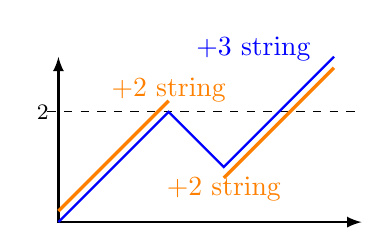
\begin{tikzpicture}[scale=.7]
                  \draw[latex-latex, thick] (0, 3) -- (0, 0) -- (5.5, 0);
                  \foreach \j in {2} {
                          \draw[dashed] (-.2, \j) -- (5.5, \j);
                          \draw (0, \j) node[left] {\footnotesize \j};
                      }
                  \draw[blue, thick] (0, 0) -- (2, 2) -- (3, 1) -- (5, 3);
                  \draw[blue] (4.75, 2.75) node[above left] {+3 string};

                  \draw[orange, very thick] (0, 0+.2) -- (2, 2+.2);
                  \draw[orange] (2,2) node[above] {+2 string};
                  \draw[orange, very thick] (3, 1-.2) -- (5, 3-.2);
                  \draw[orange] (3, 1) node[below] {+2 string};
              \end{tikzpicture}
              \caption{Decomposition of a $+3$-string into two $\pm(k+1)$-strings.}
              \label{fig:dyck_hered}
          \end{figure}
\end{itemize}

Finally, this complex algorithm has a quantum query
complexity of $O\left(\sqrt{n}(\log(n))^{0.5k}\right)$ which is a
$\tilde{\Theta}\left(\sqrt{n}\right)$. This description of the existing
algorithm stay at the surface in order to stay simple, every the pseudo
code of every subroutines can be found in
\autoref{annex:complete_subroutine_dyck_kn}. No proof of their
quantum query complexity is provided as a proof for
\autoref{th:subroutine_complexity}, almost identical,
is already provided in \autoref{proof:complexity_dyckkn}.
However, this algorithm can
be improved, indeed the first upper bound by reduction
is still better than the upper bound from algorithm.
Now, two personal improvements are described in \autoref{main_section}.
